\documentclass[12pt]{article}

% Paquetes necesarios
\usepackage[utf8]{inputenc}
\documentclass{scrartcl}
\usepackage{algorithm}
\usepackage{algpseudocode}
\usepackage{amssymb}
\usepackage[T1]{fontenc}
\usepackage[spanish]{babel}
\usepackage{graphicx}   % imágenes
\usepackage{geometry}   % márgenes
\usepackage{xcolor}     % colores
\usepackage{mdframed}   % recuadros
\usepackage{enumitem}   % listas con control
\usepackage{kantlipsum}   % alineación de texto
\geometry{margin=1.5cm}
\usepackage{amsmath}
\usepackage{listings}
\usepackage{xcolor}

\algnewcommand{\When}[1]{\State \textbf{when} #1 \textbf{do}}
\algnewcommand{\ForEach}[1]{\State \textbf{for each} #1 \textbf{do}}
\renewcommand{\qed}{\hfill\blacksquare}
\algnewcommand{\EndFor}{\State}
\newcommand{\qedwhite}{\hfill \ensuremath{\Box}}

\lstset{
  basicstyle=\ttfamily\small,
  numbers=left,
  numberstyle=\tiny,
  numbersep=8pt,
  frame=single,
  framesep=6pt,
  columns=fullflexible,
  keepspaces=true,
  showstringspaces=false,
  breaklines=true,
  escapeinside={(*@}{@*)},
  literate={<-}{{$\leftarrow$}}1
}

% Recuadro azul para ejercicios
\newmdenv[
  backgroundcolor=blue!10,
  linecolor=blue!50!black,
  linewidth=1pt,
  topline=false, bottomline=false, rightline=false,
  innertopmargin=6pt, innerbottommargin=6pt, innerleftmargin=6pt
]{ejercicio}

\begin{document}
% ---------------- ENCABEZADO CON LOGOS ----------------
\begin{center}
    \hrule
    \vspace{0.3cm}
    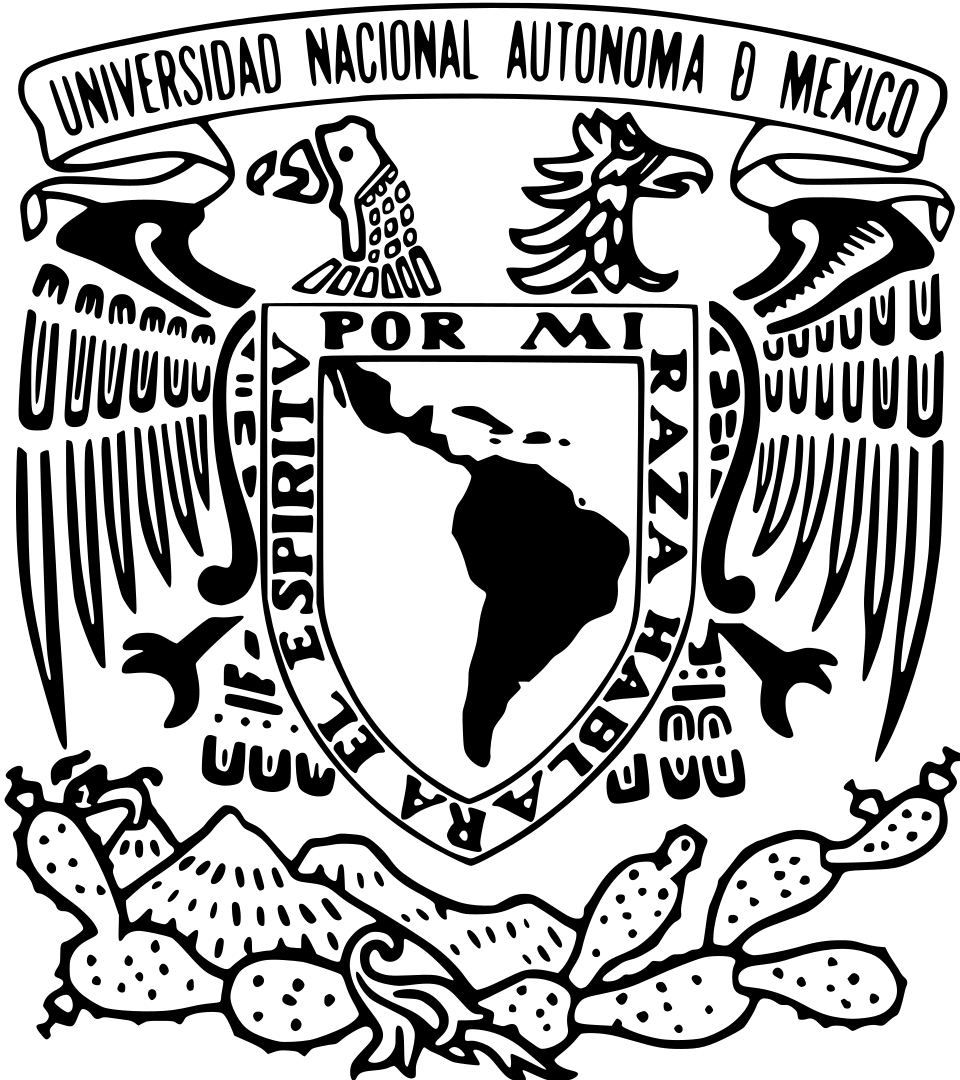
\includegraphics[width=0.15\textwidth]{img/escudo-unam.png}
    \hfill
    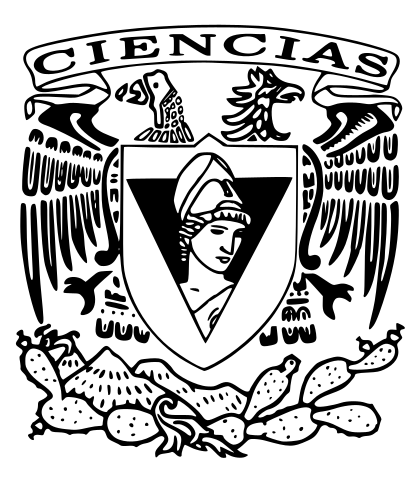
\includegraphics[width=0.15\textwidth]{img/escudo-ciencias.png}
    
    \vspace{-3cm}
    \begin{minipage}{0.7\textwidth}
        \centering
        {\medium \textbf{UNIVERSIDAD NACIONAL AUTÓNOMA DE MÉXICO}}\\[0.2cm]
        {\medium \textbf{FACULTAD DE CIENCIAS}}\\[0.2cm]
        {\medium \textbf{COMPUTACIÓN DISTRIBUIDA}}\\[0.2cm]
        {\medium \textbf{TAREA 2}}\\
    \end{minipage}
    \vspace{0.3cm}
\end{center}

\vspace{0.8cm}

% ---------------- EJERCICIOS ----------------
\begin{ejercicio}
\noindent \textbf{EJERCICIO 1.} 
Sea $G = (\Pi, E)$ un sistema distribuido síncrono. Sea $\tau$ un árbol BFS con raíz en
el proceso $p_s \in \Pi$. Demuestra que existe una ejecución del algoritmo para crear árboles
generadores que tiene como resultado $\tau$ con $p_s$ el proceso que inicia la ejecución. 
\textit{Hint:} Recuerda que en un árbol BFS, un proceso a distancia $d$ de la raíz $G$, está a distancia $d$ en $\tau$. \\
\end{ejercicio}

\noindent Usando como guía el algoritmo 5, la ejecuci\'on ocurre en un sistema distribuido s\'incrono $G = (\Pi, E)$, tomando al proceso $p_s$ como la ra\'iz del \'arbol. Inicia cuando la ra\'iz $p_s$ envia un mensaje $\text{GO}()$ a todos sus vecinos. Cuando un proceso recibe un mensaje $\text{GO}()$ por primera vez, inmediatamente designa al remitente como su padre en el \'arbol en construcci\'on. Este proceso reenv\'ia el mensaje $\text{GO}()$ a todos sus propios vecinos, excepto a su padre reci\'en asignado. Como confirmaci\'on, responde al padre con un mensaje $\text{BACK(si)}$ para aceptar la relaci\'on padre-hijo. Si un proceso ya ten\'ia un padre previamente establecido (es decir, no era su primer $\text{GO}()$), responde con un $\text{BACK(no)}$.\\

\noindent Sea $d_G(u, v)$ la distancia en el grafo original $G$ entre dos procesos $u,v$, el nivel de un proceso $p_i$ en el \'arbol BFS ser\'a $\text{nivel}(p_i) = d_G(p_s, p_i)$. Sea $L_k$ el conjunto de todos los procesos que se encuentran a una distancia $k$ de la ra\'iz $p_s$.

\begin{itemize}
    \item \textbf{Ronda 0}: La ra\'iz $p_s$ comienza el algoritmo enviando mensajes $\text{GO}() $ a sus vecinos.
    \item \textbf{Ronda $k \geq 1$}: Los procesos en el nivel $L_{k-1}$ que enviaron mensajes en la ronda anterior entregan sus mensajes. Cada proceso $p_i$ en $L_k$ que recibe su primer mensaje $\text{GO}()$ lo har\'a desde un proceso $p_j$ en $L_{k-1}$. Debido a las propiedades de BFS y de la artista entre ambos procesos, sabemos que existe $p_j$ que es el  padre de $p_i \in \tau$. Tras establecer a $p_j$ como su padre, $p_i$ actuar\'a de la siguiente manera:
    \begin{itemize}
        \item Si es una \textbf{hoja} en $\tau$ enviar\'a $\text{BACK(si)}$ a su padre.
        \item En caso contrario, enviar\'a $\text{GO}()$ a todos sus vecinos excepto a su padre.
    \end{itemize}
\end{itemize}

 \noindent Cómo es un sistema sícnrono sabemos que cualquier mensaje enviado en la ronda $r$ se recibe en la ronda $r + 1$, y que todas las acciones de los procesos en una ronda dada son ejecutados simult\'aneamente.

\noindent Así todo proceso que est\'a a una distancia $k$ de la ra\'iz en $G$ recibir\'a el mensaje $\text{GO}()$ de su futuro padre en $\tau$tal que la distancia $d$ de cada proceso a la ra\'iz en el \'arbol coincide exactamente con su distancia $d$ en el grafo original $G$ porque los mensjaes se propagan nivel a nivel. Por lo tanto, existe una ejecuci\'on de este algoritmo que genera $\tau$. $\hfill \square$

\begin{ejercicio}
\noindent \textbf{EJERCICIO 2.} 
Considere un sistema distribuido $G = (\Pi, E)$ representado como un árbol. Diseña un
algoritmo distribuido que determine la altura del árbol, es decir, la longitud del camino más
largo desde la raíz a cualquier hoja del árbol.  

\noindent \textbf{Observación.} Se puede suponer que cada proceso $p_i$ conoce su proceso padre en el árbol, y
el proceso raíz conoce su identificador único. \\
\end{ejercicio}

\begin{algorithm}
\caption{alturaArbol($p_i$)}
\begin{algorithmic}[1]
\State Variables: nodo padre, hijo; entero altura
\State Inicio:
\If{hijo = 0}
    \State envia(0) a padre
\Else
    \State altura = altura + 1
    \If{$p_i \neq$ raiz}
        \State enviar(altura) a padre
    \EndIf
\EndIf
\State Imprimir: altura del arbol = altura
\end{algorithmic}
\end{algorithm}


\begin{ejercicio}
\noindent \textbf{EJERCICIO 3.} 
Sea $G = (\Pi, E)$ un sistema distribuido asíncrono. Considera un algoritmo para construir un árbol BFS en el que sólo la raíz sabe que ya terminó la construcción del árbol. Diseña un algoritmo que le permita a cada proceso saber que ya terminó la construcción del árbol y que la raíz sepa que ya todos saben que se construyó el árbol. Argumentar por qué es correcto y la complejidad del número de mensajes y tiempo. \\
\end{ejercicio}

El problema plantea primero, construir un \'arbol BFS en un entorno as\'incrono; segundo, notificar a todos los nodos sobre la finalizaci\'on de esta construcci\'on; y tercero, confirmar en la ra\'iz que dicha notificaci\'on ha sido recibida para todos.

\begin{enumerate}
    \item Podemos aplicar el algoritmo BFS para establecer el \'arbol en el sistema as\'incrono.
    \item Usar broadcast desde la ra\'iz para informar a todos los nodos que el \'arbol est\'a completo.
    \item Utilizar unconvergecast) para que la ra\'iz reciba la confirmaci\'on de que todos los nodos tienen conocimiento del estado final.
\end{enumerate}
\newpage
\begin{algorithm}[H]
\caption{Construction BFS - Código para el proceso $p_i$}
\begin{algorithmic}[1]
\When {START is recieved}{}  \Comment{el proceso distinguido recibe el mensaje}
    \State send $GO(-1)$ to itself.

\When{$GO(d)$ is received from $p_j$}
    \If{$padre_i = \bot$}
        \State $padre_i \gets j$
        \State $hijos_i \gets \emptyset$
        \State $nivel_i \gets d+1$
        \State $mensaje\_esperado_i \gets |vecinos_i \setminus \{j\}|$
        \State $arbol \gets false$
        \If{$mensaje\_esperado_i = 0$}
            \State send $BACK(yes,d+1)$ to $p_{padre_i}$
            \State $arbol \gets true$
        \Else
            \ForEach{$k \in vecinos_i \setminus \{j\}$}
                \State send $GO(d+1)$ to $p_k$
            \State \textbf{end for}
        \EndIf
    \ElsIf{$nivel_i > d+1$}
        \State $padre_i \gets j$
        \State $hijos_i \gets \emptyset$
        \State $nivel_i \gets d+1$
        \State $mensaje\_esperado_i \gets |vecinos_i \setminus \{j\}|$
        \State $arbol\_construido\_localmente \gets false$
        \If{$mensaje\_esperado_i = 0$}
            \State send $BACK(yes,nivel_i)$ to $p_{padre_i}$
            \State $arbol \gets true$
        \Else
            \ForEach{$k \in vecinos_i \setminus \{j\}$}
                \State send $GO(d+1)$ to $p_k$
            \State \textbf{end for}
        \EndIf
    \Else
        \State send $BACK(no,d+1)$ to $p_j$
    \EndIf
\EndWhen

\When{$BACK(resp,d)$ is received from $p_j$}
    \If{$d = nivel_i + 1$}
        \If{$resp = yes$}
            \State $hijos_i \gets hijos_i \cup \{j\}$
        \EndIf
        \State $mensaje\_esperado_i \gets mensaje\_esperado_i - 1$
        \If{$mensaje\_esperado_i = 0$}
            \If{$padre_i \neq i$}
                \State send $BACK(yes,nivel_i)$ to $p_{padre_i}$
            \Else
                \State $p_i$ sabe que el árbol BFS está construido
                \State {notifica_todos ()}
            \State \textbf{end if}
            \State $arbol \gets true$
        \EndIf
    \EndIf
\EndWhen
\end{algorithmic}
\end{algorithm}

\noindent Cuando la raíz sabe que el árbol BFS está completo,notifica a todos los demás nodos.

\begin{algorithm}
\caption{Notificación}
\begin{algorithmic}[1]
\Procedure{INICIA notifica\_todos}{}
    \State $confirmaciones \gets |hijos_i|$
    \State $todos\_notificados \gets false$
    \ForEach{$j \in hijos_i$}
        \State send $AVISO\_TERMINO(nivel_i)$ to $p_j$
    \State \textbf{end for}
    \If{$confirmaciones\_pendientes = 0$}
        \State $todos\_notificados \gets true$
        \State output "Todos saben que el BFS terminó"
    \EndIf
\EndProcedure

\When{$AVISO\_TERMINO(nivel\_padre)$ is received from $p_{padre_i}$}
    \If{$nivel\_padre = nivel_i - 1$}
        \State $termino\_conocido \gets true$
        \State $confirmacione \gets |hijos_i|$
        \ForEach{$j \in hijos_i$}
            \State send $AVISO\_TERMINO(nivel_i)$ to $p_j$
        \State \textbf{end for}
        \If{$confirmaciones = 0$}
            \State send $CONFIRMACION\_TERMINO(nivel_i)$ to $p_{padre_i}$
        \EndIf
    \EndIf
\EndWhen
\end{algorithmic}
\end{algorithm}

\begin{algorithm}[H]
\caption{Confirmación de proceso terminado}
\begin{algorithmic}[1]
\When{$CONFIRMACION\_TERMINO(nivel\_hijo)$ is received from $p_j$}
    \If{$nivel\_hijo = nivel_i + 1$}
        \State $confirmaciones \gets confirmacione - 1$
        \If{$confirmaciones\_pendientes = 0$}
            \If{$padre_i \neq i$}
                \State send $CONFIRMACION\_TERMINO(nivel_i)$ to $p_{padre_i}$
            \Else
                \State $todos\_notificados \gets true$
                \State output "Todos los procesos saben que el árbol BFS está completo"
            \EndIf
        \EndIf
    \EndIf
\EndWhen
\end{algorithmic}
\end{algorithm}


\section{Complejidad del algoritmo.}
 

\noindent En la fase de construcción del árbol BFS, cada enlace de comunicación transmite como máximo un mensaje de tipo GO o BACK, lo que resulta en un total de $O(|E|)$ mensajes, donde $E$ representa el conjunto de aristas del grafo. En términos de complejidad temporal, este proceso requiere $O(D)$ unidades de tiempo, siendo $D$ el diámetro del grafo, dado que la propagación de mensajes se realiza nivel por nivel hasta alcanzar la profundidad máxima del árbol.
\begin{itemize}
    \item Para broadcast, se envía un mensaje por cada arista las aristas del árbol BFS construido. Dado que un árbol sobre $|\Pi|$ procesos contiene exactamente $|\Pi|-1$ aristas, la complejidad en mensajes es $O(|\Pi|)$. El tiempo requerido es $O(D)$ ya que la información debe propagarse desde la raíz hasta lo más profundo.

    \item Para convergecast, De manera análoga al broadcast, la confirmación de recepción emplea las $|\Pi|-1$ aristas del árbol, generando $O(|\Pi|)$ mensajes. y como el mensaje se propaga hasta lo más profundo, se tarda $O(D)$ con $D$ el diámetro de la gráfica.
\end{itemize}
Así, la complejidad en espacio sería:
\[O(|E| + |E| + |\Pi|) \in O(|E|)\]
Y la complejidad en tiempo:
\[O(|D| + |D| + |D|) \in O(|D|)\]


\begin{ejercicio}
\noindent \textbf{EJERCICIO 4.} 
Consideremos un sistema distribuido $G = (\Pi, E)$ representado como un árbol. Supongamos que cada proceso $p_i$ tiene un identificador único. Diseña un algoritmo distribuido para determinar el proceso más alejado de la raíz del árbol y la distancia de la raíz a ese proceso.

\noindent \textbf{Observación.} Puede asumir que el proceso raíz conoce su identificador único, y cada proceso $p_i$ conoce su proceso padre en el árbol. \\
\end{ejercicio}

\begin{algorithm}[H]
\caption{Encontrar el proceso más alejado($p_i$)}
\begin{algorithmic}[1]
\State \textbf{Variables locales:} $profundidad_i$, $padre_i$, $hijos_i$
\State \textbf{Broadcast INICIO:}
\If{$p_i = raíz$}
    \State $profundidad_i \gets 0$
    \State enviar $PROFUNDIDAD(0)$ a todos en $hijos_i$
\Else
    \State \textbf{al recibir} $PROFUNDIDAD(d)$ \textbf{de} $padre_i$:
    \State $profundidad_i \gets d + 1$
    \State enviar $PROFUNDIDAD(profundidad_i)$ a todos en $hijos_i$
\EndIf
\State \textbf{Convergecast:}
\If{$hijos_i = \emptyset$}
    \State enviar $(profundidad_i, i)$ a $padre_i$
\Else
    \State esperar recibir $(maxProf, idNodo)$ de cada proceso en $hijos_i$
    \State seleccionar el par $(mejorProf, mejorId)$ con el valor máximo de $maxProf$
    \If{$p_i \neq raíz$}
        \State enviar $(mejorProf, mejorId)$ a $padre_i$
    \Else
        \State \textbf{output:} `Nodo más lejano = $mejorId$, distancia = $mejorProf$`
    \EndIf
\EndIf
\end{algorithmic}
\end{algorithm}

\begin{ejercicio}
\noindent \textbf{EJERCICIO 5.} 
Sea $G = (\Pi, E)$ un sistema distribuido síncrono. Sea $M = \{m_1, m_2, \dots, m_k\}$ un conjunto de mensajes que se quieren transmitir desde un proceso $p_s$ hacia todos los demás. Debido a que el ancho de banda es muy limitado, no se puede enviar el conjunto $M$ completo, por lo que tiene que enviarse cada $m_i$ por separado. Cada proceso debe saber qué parte del mensaje está recibiendo, es decir que el $i$-ésimo mensaje es el $m_i$. Diseña un algoritmo de broadcast para diseminar $M$ sin que se repita la recepción de los mensajes en los procesos, es decir, si $p_i$ ya recibió $m_j$, no debe volver a recibirlo.  

\noindent \textit{Hint:} Broadcast sobre un árbol toma $O(n)$ mensajes porque no se repite la entrega de los mensajes. \\
\end{ejercicio}

\begin{verbatim}
Para resolver esto usaremos un algoritmo broadcast en pseudocodigo: 

Cada proceso p mantiene:
    recibido[1..k] ← false
    hijos ← lista de hijos de p en el árbol T

Proceso fuente ps:
    Para i = 1 hasta k hacer
        enviar (i, mi) a cada hijo en hijos(ps)
    Fin Para

Al recibir (i, mi) en proceso p:
    Si recibido[i] = false entonces
        recibido[i] ← true
        entregar mi a aplicación
        enviar (i, mi) a cada hijo en hijos(p)
    Sino
        ignorar mensaje
    Fin Si 
\end{verbatim}

\begin{ejercicio}
\noindent \textbf{EJERCICIO 6.} 
Sea $G = (\Pi, E)$ un sistema distribuido síncrono y sea $p_s \in \Pi$ un proceso que
empezará a ejecutar broadcast. Demuestra que broadcast no puede ejecutarse en menos de $D$
rondas, con $D$ la distancia más grande entre $p_s$ y cualquier otro proceso. \\
\end{ejercicio}
\textit{Demostración.} 
En un sistema síncrono, cada ronda permite que un mensaje avance 
a lo sumo un salto (una arista) en la red. 
Sea $D = \max_{v \in \Pi} \mathrm{dist}(p_s,v)$, es decir, la excentricidad de $p_s$. 

Podemos definir $S_k$ como el conjunto de nodos que conocen el mensaje 
al final de la ronda $k$. Claramente $S_0 = \{p_s\}$. 
Supongamos por inducción que todo nodo en $S_k$ está a distancia 
menor o igual que $k$ de $p_s$. 
En la ronda $k+1$, únicamente los vecinos de nodos en $S_k$ 
pueden recibir el mensaje, y cualquier vecino de un nodo 
a distancia $\leq k$ está a distancia $\leq k+1$ de $p_s$. 
Así, todos los nodos en $S_{k+1}$ están a distancia 
menor o igual que $k+1$ de $p_s$. 

Por inducción, concluimos que, después de $k$ rondas, 
únicamente los nodos con distancia $\mathrm{dist}(p_s,v) \leq k$ 
pueden conocer el mensaje. 

Ahora sea $v \in \Pi$ con $\mathrm{dist}(p_s,v) = D$. 
Si existiera un algoritmo de \textit{broadcast} que terminara en 
menos de $D$ rondas, entonces $v$ debería conocer el mensaje antes, 
lo cual contradice el resultado anterior. 

Por tanto, ningún algoritmo de \textit{broadcast} puede ejecutarse 
en menos de $D$ rondas. 

\begin{ejercicio}
\noindent \textbf{EJERCICIO 7.} 
En la CDMX varios puntos de control (nodos) fueron agregados. Cada uno de
estos puntos tiene información sobre el número de personas que viven dentro de cierto diámetro.
Un punto (raíz) de la delegación Benito Juárez quiere recolectar la información de todos los puntos de control y determinar cuántas personas viven en la CDMX. Escribe un algoritmo distribuido para que cada nodo recolecte la información de sus hijos para enviársela al padre sin repetirla y que el padre reporte el total de pobladores viviendo en la CDMX. \\
\end{ejercicio}
Para resolver este problema usaremos el algoritmo convergecast. En donde Cada nodo espera los resultados de sus hijos, los suma con su propio valor local 
y envía el resultado a su padre. La raíz obtiene finalmente el total.

\textbf{Algoritmo ConvergecastCDMX}
\begin{enumerate}
  \item Cada nodo $u$ conoce su valor local $\text{personas}[u]$.
  \item El nodo $u$ espera hasta recibir un mensaje \texttt{SUMA} de cada uno de sus hijos.
  \item Entonces calcula:
  \[
    \text{total}_u \leftarrow \text{personas}[u] 
      + \sum_{\text{hijo } v \text{ de } u} \text{total}_v
  \]
  \item Si $u$ no es la raíz, envía el mensaje 
  \texttt{SUMA}$(\text{total}_u)$ a su padre.
  \item Si $u$ es la raíz, reporta $\text{total}_u$ como el número de 
  personas que viven en la CDMX.
\end{enumerate}

\medskip

\textit{Correctitud.} Dado que la topología es un árbol, cada nodo tiene un único padre, 
por lo que su información se transmite una sola vez y no se repite. 
Al final, la raíz obtiene la suma de todos los valores.

\medskip

\textit{Complejidad.} 
\begin{itemize}
  \item \textbf{Mensajes:} se envía exactamente un mensaje por arista, 
  por lo que el costo total es $O(|\Pi|)$. 
  \item \textbf{Tiempo:} $O(\{altura del árbol})$ rondas síncronas.
\end{itemize}



\begin{ejercicio}
\noindent \textbf{EJERCICIO 8.} 
Considera el algoritmo de convergecast sobre el árbol generador ya construido.
Demuestra que cualquier nodo a altura $h$ (distancia más corta desde la hoja hacia el nodo)
envía un mensaje a más tardar en la ronda $h$. \\
\end{ejercicio}

\textit{Demostración.} Sea la altura de un nodo $u$ definida como
\[
h(u) = \min_{l \in \text{Hojas}} \mathrm{dist}(u,l).
\]

\textbf{Afirmación.} Un nodo a altura $h$ envía su mensaje a más tardar en la ronda $h$.

\medskip

\textbf{Base: $h=0$.}  
Si $u$ es una hoja, entonces no tiene hijos y puede enviar inmediatamente 
su valor local a su padre en la primera ronda. 
Así, toda hoja envía en la ronda $1 \leq 0+1$.

\medskip

\textbf{Paso inductivo.}  
Supongamos que todo nodo de altura $h-1$ envía su mensaje a más tardar en 
la ronda $h-1$. Sea $u$ un nodo de altura $h$.  
\begin{itemize}
  \item Los hijos de $u$ tienen altura menor o igual que $h-1$.  
  \item Por hipótesis inductiva, cada hijo envía su mensaje a más tardar en la ronda $h-1$.  
  \item Entonces $u$ recibe todos los mensajes de sus hijos a más tardar en la ronda $h-1$.  
  \item En la siguiente ronda ($h$), $u$ puede sumar sus valores y enviar su mensaje a su padre.  
\end{itemize}

\medskip

\textbf{Conclusión.}  
Por inducción, todo nodo a altura $h$ envía su mensaje a más tardar en la ronda $h$.  

\end{document}

